\documentclass[conference]{IEEEtran}
\IEEEoverridecommandlockouts
\usepackage{cite}
\usepackage{amsmath,amssymb,amsfonts}
\usepackage{algorithmic}
\usepackage{graphicx}
\usepackage{textcomp}
\usepackage{xcolor}
\usepackage{url}
\usepackage{breakurl}
\renewcommand{\refname}{Referências}
\renewcommand{\tablename}{Tabela}
\renewcommand{\figurename}{Fig.}

\usepackage{hyperref}

\hypersetup{
    colorlinks=true,
    linkcolor=blue,
    citecolor=blue,
    urlcolor=blue,
    allcolors=blue
}

\begin{document}

\title{Integração de um acelerador ISFFT ao processador NEORV32 (RISC-V): verificação UVM, DFT, prototipagem em FPGA e fluxo ASIC até o GDSII em SkyWater 130 nm}

\author{\IEEEauthorblockN{Lukas Araújo da Silva}
\IEEEauthorblockA{\textit{Engenharia Eletrônica} \\
\textit{Universidade de Brasília (UnB)}\\
Brasília, Brasil \\
lukas.araujo.cp@gmail.com}
}

\maketitle

\begin{abstract}
Este relatório descreve a etapa final do projeto do Programa CI Digital (MCTI/Softex). O módulo \textit{Inverse Symplectic Finite Fourier Transform} (ISFFT), desenvolvido no Estudo Dirigido 1 para a modulação \textit{Orthogonal Time Frequency Space} (OTFS) em enlaces com satélites LEO, foi integrado como periférico do processador RISC-V NEORV32. O IP foi verificado com a metodologia UVM no Cadence Xcelium: 10 testes aprovados, 9.928 palavras comparadas bit a bit, 100\% de cobertura funcional e 8 de 8 asserções. Recebeu também cadeias de varredura (\textit{scan}) e padrões de ATPG gerados no Cadence Modus, com 99,65\% de cobertura de falhas \textit{stuck-at} em 170 padrões e um custo de 17,2\% em área de lógica. O sistema NEORV32 + ISFFT foi prototipado na Kria KR260 a 100 MHz, onde o processador RISC-V controla sozinho o DMA e o acelerador, com latência de 6,87 $\mu$s por matriz e EVM idêntico ao modelo de referência (3,41/0,78/0,60\%). Para o fluxo ASIC, a arquitetura foi adaptada com memórias geradas pela OpenRAM e sintetizada no Cadence Genus em SkyWater 130 nm: 1,91 mm$^2$, folga de +2,41 ns a 50 MHz, equivalência formal confirmada no Conformal e simulação pós-síntese idêntica ao RTL. Como atividade extra, o netlist foi levado ao GDSII com ferramentas abertas (LibreLane/OpenROAD), incluindo o anel de \textit{pads}, com DRC e LVS limpos.
\end{abstract}

\begin{IEEEkeywords}
OTFS, ISFFT, RISC-V, NEORV32, UVM, DFT, ATPG, FPGA, Kria KR260, ASIC, SkyWater 130 nm, OpenRAM, LibreLane.
\end{IEEEkeywords}

% =====================================================================
\section{Introdução}

\subsection{O Efeito Doppler em Enlaces com Satélites LEO}
Constelações de satélites em órbita baixa (LEO) oferecem conectividade com baixa latência em qualquer ponto do planeta, mas o satélite se desloca a cerca de 7,5 km/s em relação à estação terrena. Como ilustra a Fig.~\ref{fig_sat}, o sinal recebido sofre um desvio de frequência $\Delta f$ que muda de sinal durante a passagem:

\begin{equation}
\Delta f = \frac{v}{c}\, f_0 ,
\end{equation}

\noindent o que resulta em cerca de $\pm 50$ kHz para uma portadora de 2 GHz e $\pm 300$ kHz em 12 GHz (banda Ku). Esses valores superam o espaçamento de 15 kHz entre subportadoras do OFDM usado no LTE e no 5G. A modulação OFDM perde então a ortogonalidade entre subportadoras, surge Interferência Inter-Canal (ICI) e o canal varia dentro de um mesmo quadro, o que exige equalização complexa e muitos pilotos \cite{b1}\cite{b2}.

\begin{figure}[htbp]
\centerline{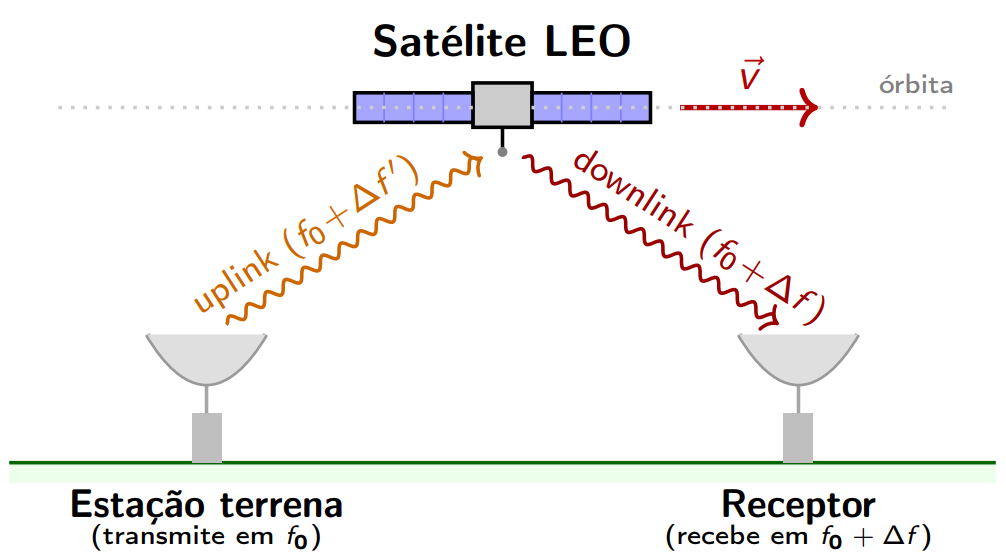
\includegraphics[width=0.46\textwidth]{Imagens/doppler_satelite.png}}
\caption{Desvio Doppler em um enlace com satélite LEO: a frequência recebida $f_0+\Delta f$ depende da velocidade relativa entre o satélite e a estação.}
\label{fig_sat}
\end{figure}

\subsection{O Domínio Atraso-Doppler}
A modulação OTFS organiza os símbolos de informação em uma grade bidimensional no domínio atraso-Doppler, cujos eixos representam o tempo de chegada ($\tau$) e a velocidade relativa ($\nu$) de cada refletor (Fig.~\ref{fig_channel}). Nesse domínio, cada caminho de propagação é um ponto: o canal é esparso e permanece quase constante durante o quadro. Cada símbolo se espalha por todo o quadro tempo-frequência e experimenta a diversidade completa do canal. Assim, o OTFS não elimina o Doppler: ele o representa de forma que o receptor consiga separá-lo \cite{b1}\cite{b3}.

\begin{figure}[htbp]
\centerline{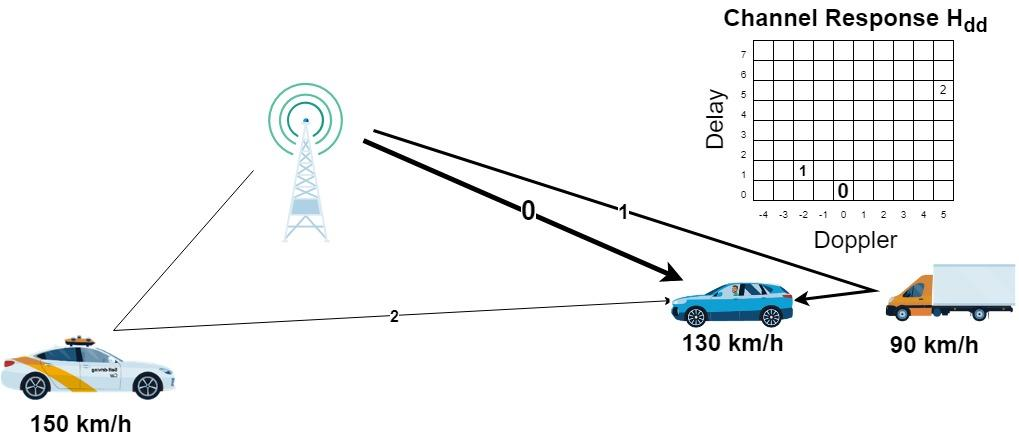
\includegraphics[width=0.48\textwidth]{Imagens/doppler_domain.png}}
\caption{Representação física do canal no domínio atraso-Doppler, adaptado de \cite{b2}.}
\label{fig_channel}
\end{figure}

\subsection{A ISFFT no Transmissor OTFS}
A ISFFT converte a grade de símbolos $X_{dd}[k,l]$ do domínio atraso-Doppler para a grade tempo-frequência $X_{tf}[n,m]$, que segue para a transformada de Heisenberg, equivalente a um modulador OFDM (Fig.~\ref{fig_otfs_chain}). Para uma matriz $N \times M$ ($8 \times 8$ neste trabalho) \cite{b3}:

\begin{equation}
X[n, m] = \frac{1}{\sqrt{NM}} \sum_{k=0}^{N-1} \sum_{l=0}^{M-1} X[k, l]\, e^{j2\pi(\frac{nk}{N} - \frac{ml}{M})}
\label{eq_isfft}
\end{equation}

A transformada é separável: equivale a uma IFFT de $N$ pontos ao longo de um eixo seguida de uma FFT de $M$ pontos ao longo do outro. Essa propriedade define a arquitetura em hardware, com dois núcleos unidimensionais e uma memória de transposição entre eles.

\begin{figure*}[htbp]
\centerline{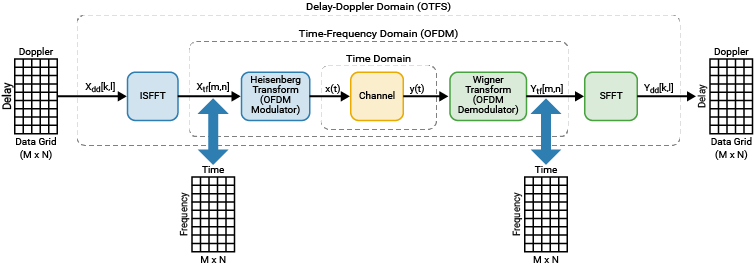
\includegraphics[width=0.85\textwidth]{Imagens/OTFS_diagram.png}}
\caption{Cadeia de modulação OTFS com os domínios atraso-Doppler e tempo-frequência, adaptado de \cite{b2}. A ISFFT é o pré-processador do transmissor.}
\label{fig_otfs_chain}
\end{figure*}

\subsection{Objetivos}
O objetivo desta etapa é implementar o IP ISFFT desenvolvido no Estudo Dirigido 1 \cite{b14} como periférico do processador NEORV32 \cite{b5}, validando o IP com UVM e DFT, o sistema na FPGA Kria KR260 e o fluxo ASIC até o GDSII. Os objetivos específicos são:
\begin{itemize}
    \item Verificar o IP ISFFT com um ambiente UVM, com relatório de funcionalidade e de cobertura.
    \item Inserir cadeias de \textit{scan} no IP e gerar padrões de teste por ATPG.
    \item Integrar o IP ao NEORV32 na Kria KR260, com o processador RISC-V controlando o acelerador e o DMA.
    \item Adaptar o sistema para ASIC em SkyWater 130 nm e realizar a síntese, a simulação pós-síntese e a verificação de equivalência no Cadence.
    \item Como atividade extra, levar o netlist sintetizado até o GDSII com ferramentas abertas.
\end{itemize}

% =====================================================================
\section{Arquitetura e Metodologia}

\subsection{Fluxos de Desenvolvimento e Ferramentas}
O trabalho seguiu dois fluxos. No \textbf{fluxo embarcado}, o RTL do NEORV32 (VHDL) e da ISFFT (Verilog) foi integrado no Vivado, o firmware do RISC-V foi compilado com o \textit{riscv-none-elf-gcc} e a validação foi feita por \textit{hardware-in-the-loop} com o PYNQ, como no Estudo Dirigido 1. No \textbf{fluxo ASIC}, a parte 1 usa o Cadence (síntese, simulação pós-síntese, equivalência, UVM e DFT) e a parte 2, extra, usa ferramentas abertas para o layout. A divisão é necessária porque o ambiente Cadence disponível não tem as regras físicas do SkyWater 130 nm para DRC, LVS e extração. A Tabela~\ref{tab_tools} resume as ferramentas.

\begin{table}[htbp]
\caption{Ferramentas utilizadas em cada etapa}
\label{tab_tools}
\begin{center}
\resizebox{\columnwidth}{!}{%
\begin{tabular}{|l|l|}
\hline
\textbf{Etapa} & \textbf{Ferramenta (versão)} \\
\hline
Prototipagem em FPGA & Vivado, PYNQ (Kria KR260) \\
Síntese lógica & Cadence Genus 22.16 \\
Simulação RTL e pós-síntese & Cadence Xcelium 23.09 \\
Verificação UVM e cobertura & Cadence Xcelium 26.03, IMC 26.03 \\
Equivalência formal (LEC) & Cadence Conformal 23.2 e 26.1 \\
ATPG & Cadence Modus 25.1 \\
Macros de memória & OpenRAM 1.2.49 \\
NEORV32: VHDL $\rightarrow$ Verilog & GHDL \\
Layout (extra) & LibreLane 3.0.14 (OpenROAD, Magic, Netgen, KLayout) \\
\hline
\end{tabular}%
}
\end{center}
\end{table}

\subsection{O IP ISFFT}
O núcleo do IP é o mesmo do Estudo Dirigido 1 (Fig.~\ref{fig_pipeline}). Dois núcleos de 8 pontos gerados pelo Spiral \cite{b4}, com representação em ponto fixo de 16 bits para as partes real e imaginária, latência de 41 ciclos e uma transformada a cada 4 ciclos, realizam a IFFT nas linhas e a FFT nas colunas. Entre eles, um banco \textit{ping-pong} de $2 \times 8 \times 8$ palavras de 32 bits faz a transposição: uma matriz é escrita por linhas em um banco enquanto a anterior é lida por colunas do outro. O modelo de referência em Python aplica \textit{ifft} nas linhas, \textit{fft} nas colunas e divide o resultado por 8.

\begin{figure*}[htbp]
\centerline{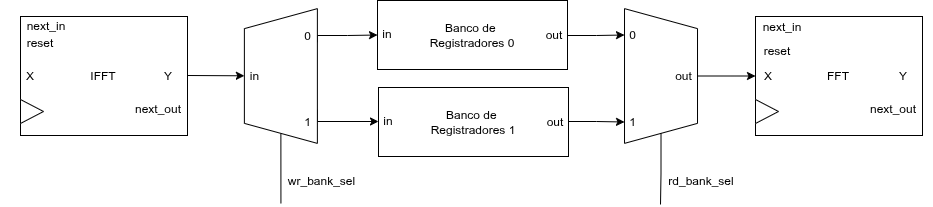
\includegraphics[width=0.85\textwidth]{Imagens/Pipeline.png}}
\caption{Bloco operacional da ISFFT: IFFT 1D, banco \textit{ping-pong} de transposição e FFT 1D.}
\label{fig_pipeline}
\end{figure*}

Para ser controlado pelo RISC-V, o núcleo recebeu um invólucro (\textit{wrapper}) com três interfaces: AXI-Stream de entrada e de saída para os dados e AXI4-Lite para o controle. Cada palavra de 64 bits carrega duas amostras complexas, portanto uma matriz $8 \times 8$ ocupa 32 palavras. O \textit{wrapper} contém:
\begin{itemize}
    \item \textbf{Buffer de entrada} de 64 palavras com \textit{commit}/\textit{rollback}: a matriz só é confirmada após 32 palavras; um \texttt{tlast} prematuro descarta a matriz truncada sem travar o núcleo.
    \item \textbf{Liberador por crédito}: só entrega uma matriz ao núcleo se houver espaço reservado na saída, de modo que nenhum resultado seja perdido.
    \item \textbf{FIFO de saída} de 256 palavras, que respeita o \texttt{tready} (contrapressão) e gera o \texttt{tlast} a cada \texttt{PKT\_MAT} matrizes.
\end{itemize}
Os registradores AXI4-Lite estão na Tabela~\ref{tab_regs}. Na versão ASIC (\texttt{isfft\_axi\_v4}), o buffer de entrada e a FIFO de saída passaram a ser macros SRAM, o que exigiu uma pré-busca, porque a macro só oferece leitura síncrona.

\begin{table}[htbp]
\caption{Mapa de registradores AXI4-Lite do IP}
\label{tab_regs}
\begin{center}
\resizebox{\columnwidth}{!}{%
\begin{tabular}{|c|l|l|}
\hline
\textbf{Offset} & \textbf{Registrador} & \textbf{Função} \\
\hline
0x00 & CTRL (R/W) & \textit{enable}, \textit{soft reset}, limpeza de erros \\
0x04 & STATUS (RO) & ocupado, FIFO cheia/com dados, erros \\
0x08 & MAT\_IN (RO) & matrizes confirmadas na entrada \\
0x0C & MAT\_OUT (RO) & matrizes entregues na saída \\
0x10 & ERR\_CNT (RO) & erros de \texttt{tlast} \\
0x14 & ID (RO) & identificação \texttt{0x15FF0300} \\
0x18 & PKT\_MAT (R/W) & matrizes por pacote de saída \\
\hline
\end{tabular}%
}
\end{center}
\end{table}

\subsection{Arquitetura com o NEORV32 na Kria KR260}
Na Kria (Fig.~\ref{fig_kria_arch}), o NEORV32 é o controlador do SoC na lógica programável (PL). Ele configura a ISFFT pelo AXI4-Lite e programa um AXI DMA que lê a matriz da memória DDR, a envia pelo AXI-Stream à ISFFT e grava o resultado de volta. O firmware e uma caixa de correio ficam em uma BRAM de 64 kB. O sistema de processamento (PS), com o ARM Cortex-A53 rodando Ubuntu e PYNQ, apenas carrega o \textit{bitstream} e o firmware, aloca os buffers na DDR e serve como depurador. O \textit{block design} correspondente está na Fig.~\ref{fig_bd}.

\begin{figure}[htbp]
\centerline{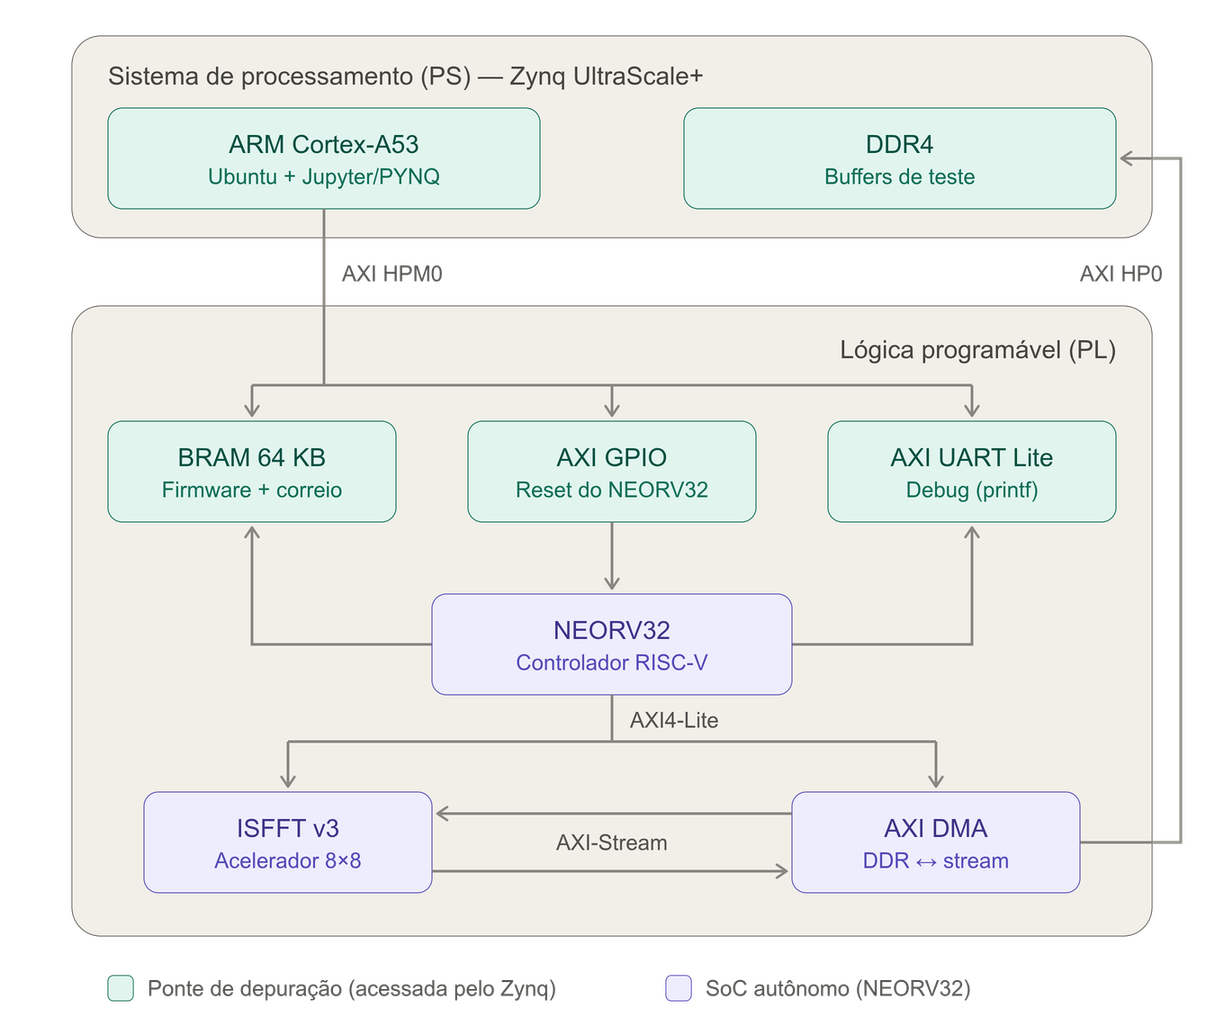
\includegraphics[width=0.40\textwidth]{Imagens/kria_neorv32.png}}
\caption{Arquitetura na Kria KR260: o NEORV32 controla a ISFFT e o AXI DMA; o Zynq atua como ponte de depuração.}
\label{fig_kria_arch}
\end{figure}

\begin{figure*}[htbp]
\centerline{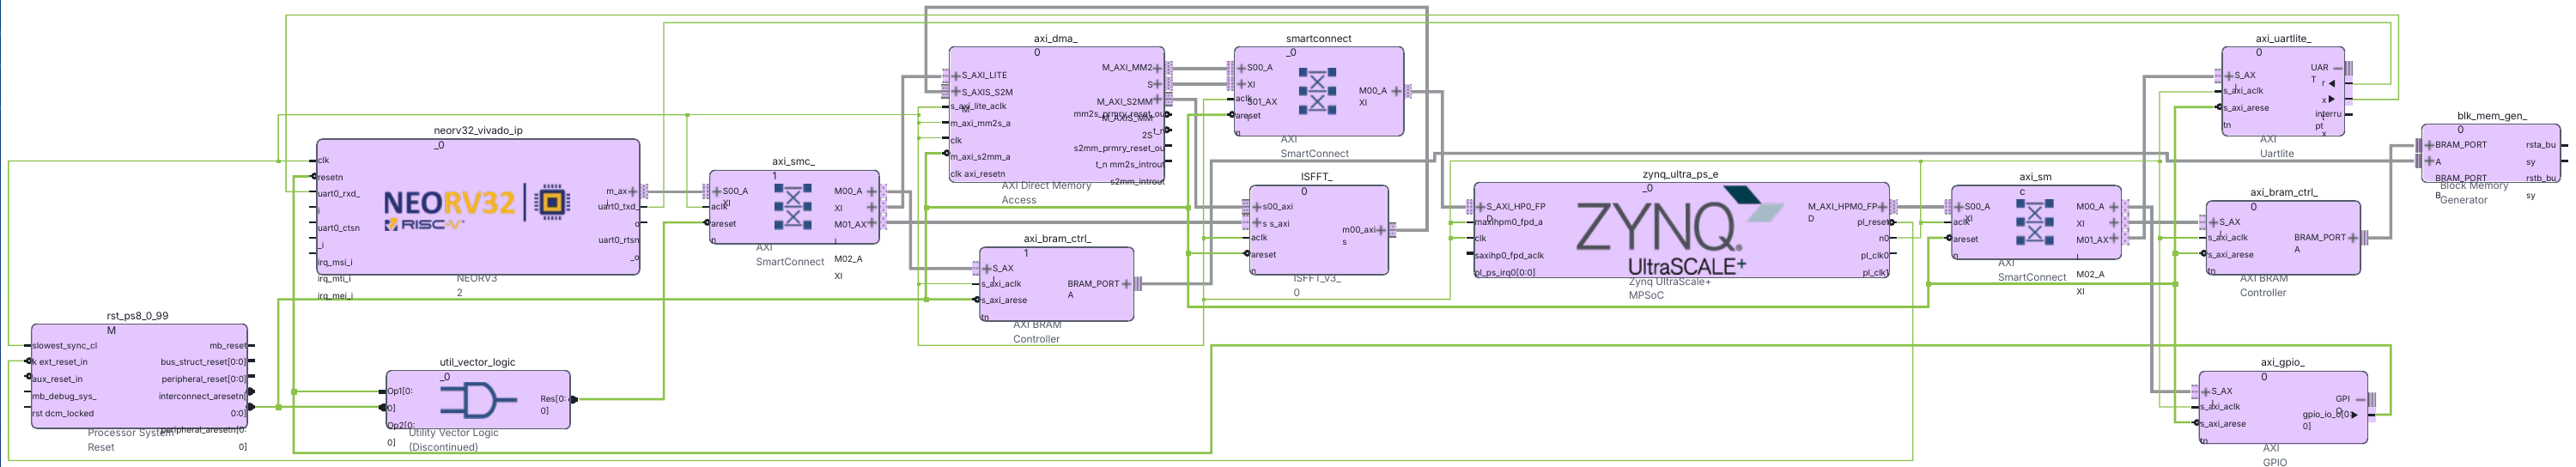
\includegraphics[width=0.98\textwidth]{Imagens/block_design_neorv32.png}}
\caption{\textit{Block design} no Vivado com o NEORV32, a ISFFT, o AXI DMA, as BRAMs e o Zynq UltraScale+.}
\label{fig_bd}
\end{figure*}

\subsection{Arquitetura com o NEORV32 no ASIC}
Em ASIC não existem o Zynq, o AXI DMA e os demais IPs da Xilinx. A arquitetura foi adaptada como mostra a Fig.~\ref{fig_asic_arch}:
\begin{itemize}
    \item O NEORV32 (rv32imc) é o único processador; o programa fica na IMEM, carregada pelo \textit{testbench}.
    \item O DMA e o SLINK do próprio NEORV32 movem os dados. A FIFO do SLINK tem 64 posições, o suficiente para uma matriz inteira, e conversores de 32 para 64 bits ligam o SLINK à ISFFT.
    \item Uma ponte XBUS $\rightarrow$ AXI4-Lite dá acesso aos registradores do IP.
    \item O NEORV32 foi convertido de VHDL para um único Verilog com o GHDL, porque o fluxo aberto não lê VHDL.
    \item O relógio passou de 100 para 50 MHz, e o banco de registradores da CPU foi implementado em \textit{flip-flops}.
\end{itemize}

\begin{figure}[htbp]
\centerline{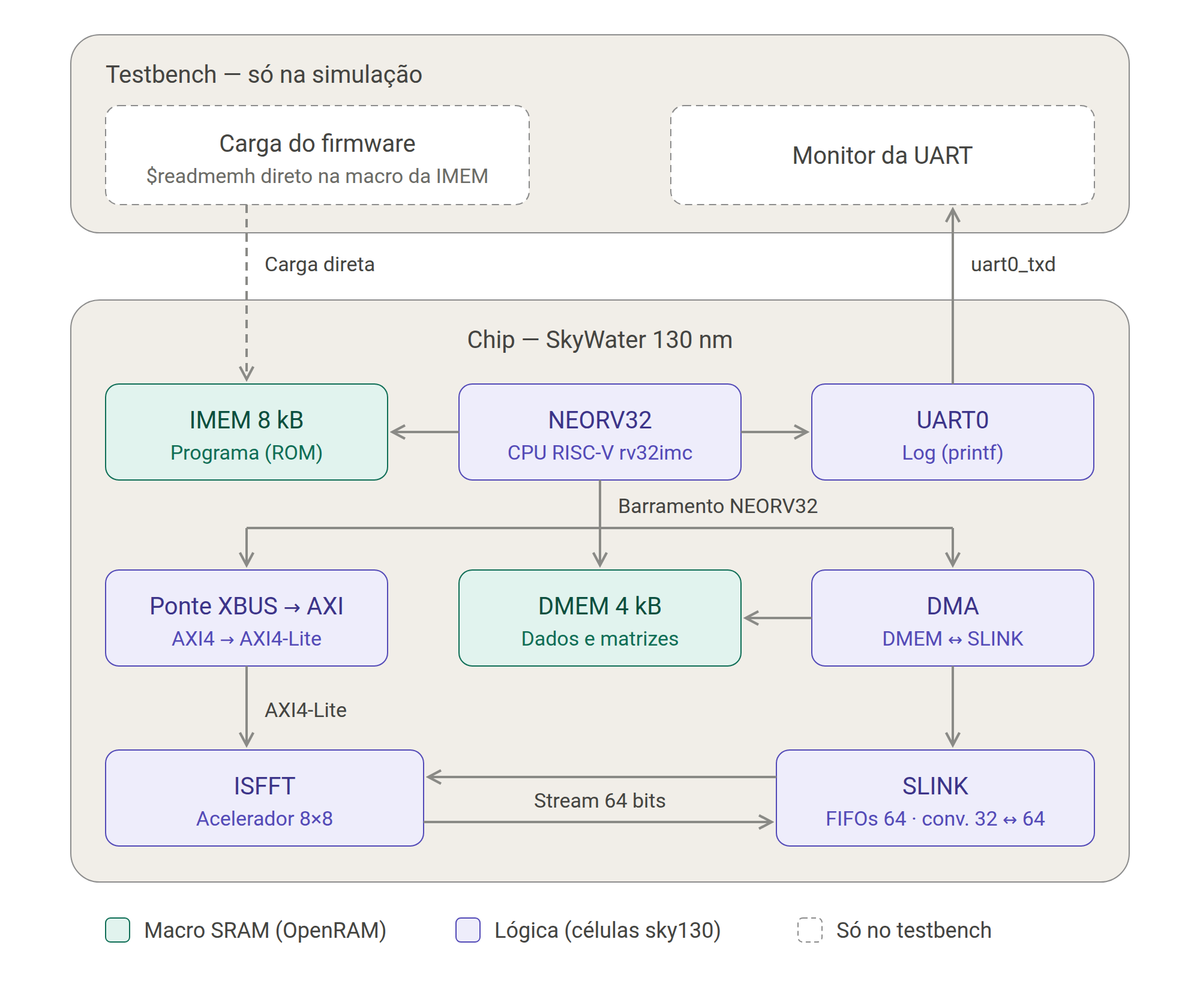
\includegraphics[width=0.44\textwidth]{Imagens/asic_neorv32.png}}
\caption{Arquitetura do SoC em ASIC: IMEM e DMEM em macros OpenRAM, transporte de dados por DMA e SLINK do NEORV32.}
\label{fig_asic_arch}
\end{figure}

\subsection{Tecnologia: SkyWater 130 nm e OpenRAM}
O PDK SkyWater 130 nm \cite{b6} é aberto (licença Apache 2.0) e traz tudo de que o fluxo aberto precisa para chegar ao GDSII: LEF, Liberty, GDS e as regras do Magic, do Netgen e do KLayout. Não exige NDA, de modo que layout, macros e documentação podem ser publicados. Foi usada a biblioteca de alta densidade \texttt{sky130\_fd\_sc\_hd} a 1,8 V, com cinco camadas de metal (met1 a met5) além da camada \textit{li1}.

O PDK aberto não inclui compilador de memória da \textit{foundry}. As memórias grandes foram geradas pela OpenRAM \cite{b7}, um compilador aberto que, a partir de um arquivo de configuração (largura da palavra, profundidade, portas, escrita por byte), produz a macro completa: GDS, LEF, Liberty, Verilog e SPICE (Fig.~\ref{fig_macro}). Uma memória em \textit{flip-flops} custa cerca de 43,9 $\mu$m$^2$/bit, contra 8,7 $\mu$m$^2$/bit na macro de 4 kB. Uma macro de duas portas (1rw1r) de 64 bits, porém, tem um custo fixo de cerca de 103.900 $\mu$m$^2$ mais 11,8 $\mu$m$^2$/bit, e por isso só compensa acima de aproximadamente 3.200 bits. Essa regra, medida com macros de vários tamanhos, definiu a implementação de cada memória (Tabela~\ref{tab_mem}): quatro macros no total. O número de macros é ditado também pelos acessos por ciclo, e não só pelos bits: o \textit{ping-pong} faz duas leituras e duas escritas por ciclo.

\begin{figure}[htbp]
\centerline{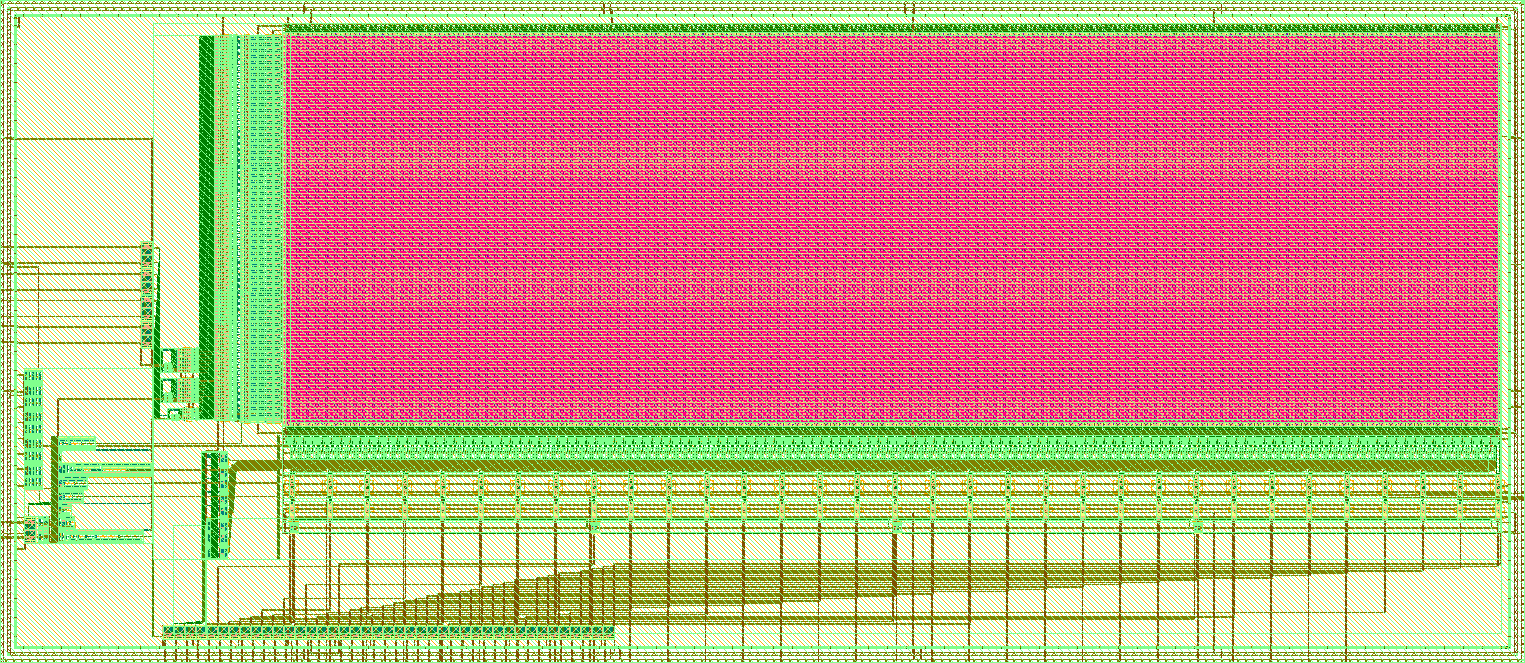
\includegraphics[width=0.46\textwidth]{Imagens/macro_4kb.png}}
\caption{Layout da macro OpenRAM de 4 kB (DMEM), $808{,}8 \times 351{,}3$ $\mu$m: matriz de \textit{bitcells} e periferia gerada pela OpenRAM.}
\label{fig_macro}
\end{figure}

\begin{table}[htbp]
\caption{Implementação das memórias do SoC}
\label{tab_mem}
\begin{center}
\resizebox{\columnwidth}{!}{%
\begin{tabular}{|l|c|l|r|}
\hline
\textbf{Memória} & \textbf{Tamanho} & \textbf{Implementação} & \textbf{Área ($\mu$m$^2$)} \\
\hline
IMEM (programa) & $2048 \times 32$ & Macro 1rw 8 kB & 448.827 \\
DMEM (dados) & $1024 \times 32$ & Macro 1rw 4 kB & 284.139 \\
FIFO de saída da ISFFT & $256 \times 64$ & Macro 1rw1r & 296.939 \\
Buffer de entrada da ISFFT & $64 \times 64$ & Macro 1rw1r & 152.932 \\
\textit{Ping-pong} da ISFFT & $2 \times 8 \times 8 \times 32$ & \textit{Flip-flops} & -- \\
Memórias internas do Spiral & $16 \times (4~\text{ou}~8) \times 32$ & \textit{Flip-flops} & -- \\
FIFOs do SLINK, DMA e UART & $\leq 64 \times 37$ & \textit{Flip-flops} & -- \\
\hline
\end{tabular}%
}
\end{center}
\end{table}

\subsection{Estratégia de Validação: as Três Matrizes de Teste}
Desde o Estudo Dirigido 1, as mesmas três matrizes de entrada são usadas em todas as etapas: um impulso na posição [3,3] com amplitude 1000, uma senoide 2D com amplitude 500 e uma rampa com valor $10 \times$ índice (Fig.~\ref{fig_input}). A precisão é medida pelo \textit{Error Vector Magnitude} contra o modelo em ponto flutuante:

\begin{equation}
\text{EVM} = \sqrt{\frac{\text{média}\,|X_{hw}-X_{ref}|^2}{\text{média}\,|X_{ref}|^2}} \times 100\%
\end{equation}

No sistema ASIC, o firmware do NEORV32 calcula também uma soma de verificação de cada uma das três saídas. Usar sempre o mesmo estímulo torna qualquer divergência visível de imediato. A Tabela~\ref{tab_fio} resume onde esse estímulo foi aplicado ao longo do projeto.

\begin{figure*}[htbp]
\centerline{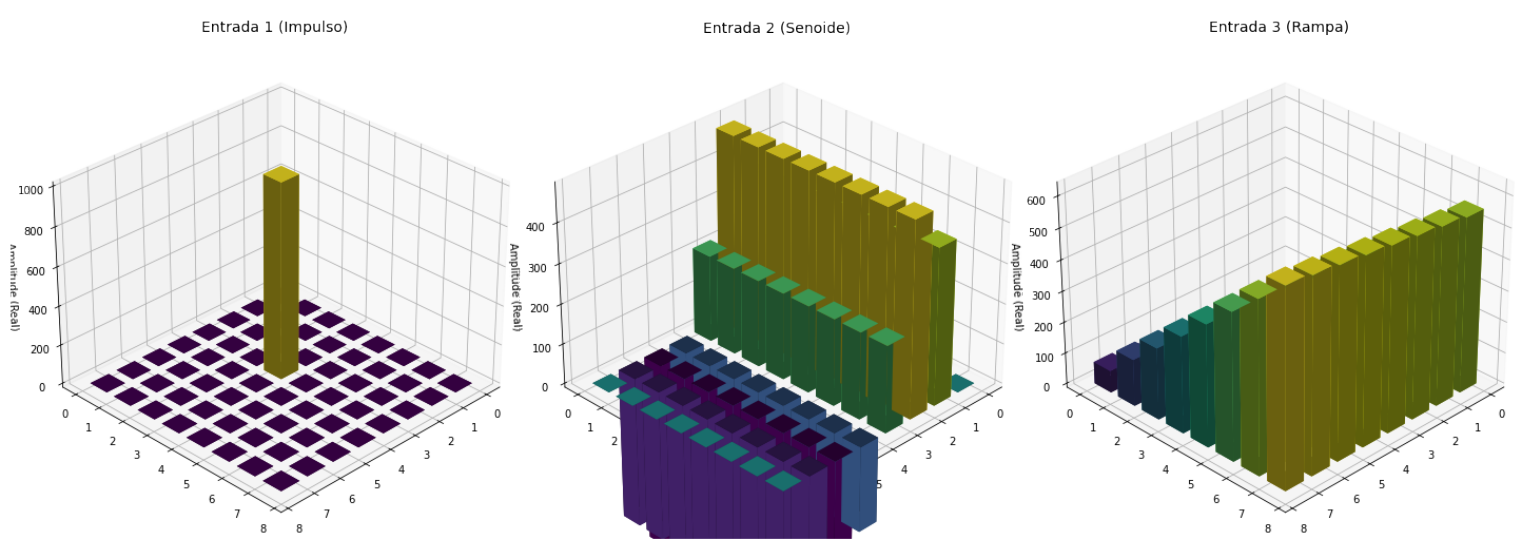
\includegraphics[width=0.85\textwidth]{Imagens/graph1.png}}
\caption{Matrizes de entrada $8 \times 8$ usadas em todas as etapas: impulso, senoide e rampa.}
\label{fig_input}
\end{figure*}

\begin{table}[htbp]
\caption{As três matrizes ao longo do projeto}
\label{tab_fio}
\begin{center}
\begin{tabular}{|l|l|}
\hline
\textbf{Etapa} & \textbf{Resultado} \\
\hline
Kria KR260 (placa) & EVM 3,4122 / 0,7822 / 0,5965\% \\
Simulação RTL do SoC & EVM idêntico à placa \\
UVM (teste \texttt{kria}) & EVM idêntico à placa \\
Pós-síntese (Genus) & 3 somas iguais ao RTL \\
Netlist do layout & 3 somas iguais ao RTL \\
Chip com os \textit{pads} & 3 somas iguais ao RTL \\
\hline
\end{tabular}
\end{center}
\end{table}

% =====================================================================
\section{Verificação do IP com UVM}

\subsection{Proposta do Ambiente}
O ambiente UVM (Fig.~\ref{fig_uvm}) verifica apenas o IP, sem o processador. O DUT é o \texttt{isfft\_axi\_v4}, o mesmo RTL sintetizado no Cadence, com os modelos das duas macros SRAM. O ambiente é composto por:
\begin{itemize}
    \item \textbf{Agentes} AXI4-Lite e AXI-Stream de entrada e de saída, com atrasos, pausas e contrapressão sorteados (\texttt{tready} entre 50 e 100\% e paradas longas).
    \item \textbf{RAL} com os 7 registradores; os contadores são previstos pelo modelo e conferidos.
    \item \textbf{Modelo de referência} que reproduz o \textit{commit}/\textit{rollback} da entrada e passa cada matriz pelo \textit{wrapper} validado na etapa 1.
    \item \textbf{\textit{Scoreboard}} com duas checagens independentes: bit a bit contra o modelo de referência e numérica contra a ISFFT em ponto flutuante, com tolerância de 4 LSB, além de um modelo do \texttt{tlast}.
    \item \textbf{Oito asserções} ligadas ao DUT por \texttt{bind}, sem alterar o RTL, e checagem de protocolo AXI nas interfaces.
    \item \textbf{Cobertura funcional} em 4 grupos com 54 \textit{bins}: entrada, saída, registradores e ocupação dos buffers.
\end{itemize}
A simulação usou o Xcelium 26.03 com UVM 1.1d \cite{b10} a 50 MHz. Antes de usar a máquina com as licenças, o ambiente foi conferido no Verilator 5.052 com 12 defeitos plantados no RTL: todos foram detectados. Os dois defeitos inseridos no núcleo Spiral só foram vistos pela checagem numérica, porque a referência bit a bit usa o mesmo núcleo; isso justifica manter as duas checagens.

\begin{figure}[htbp]
\centerline{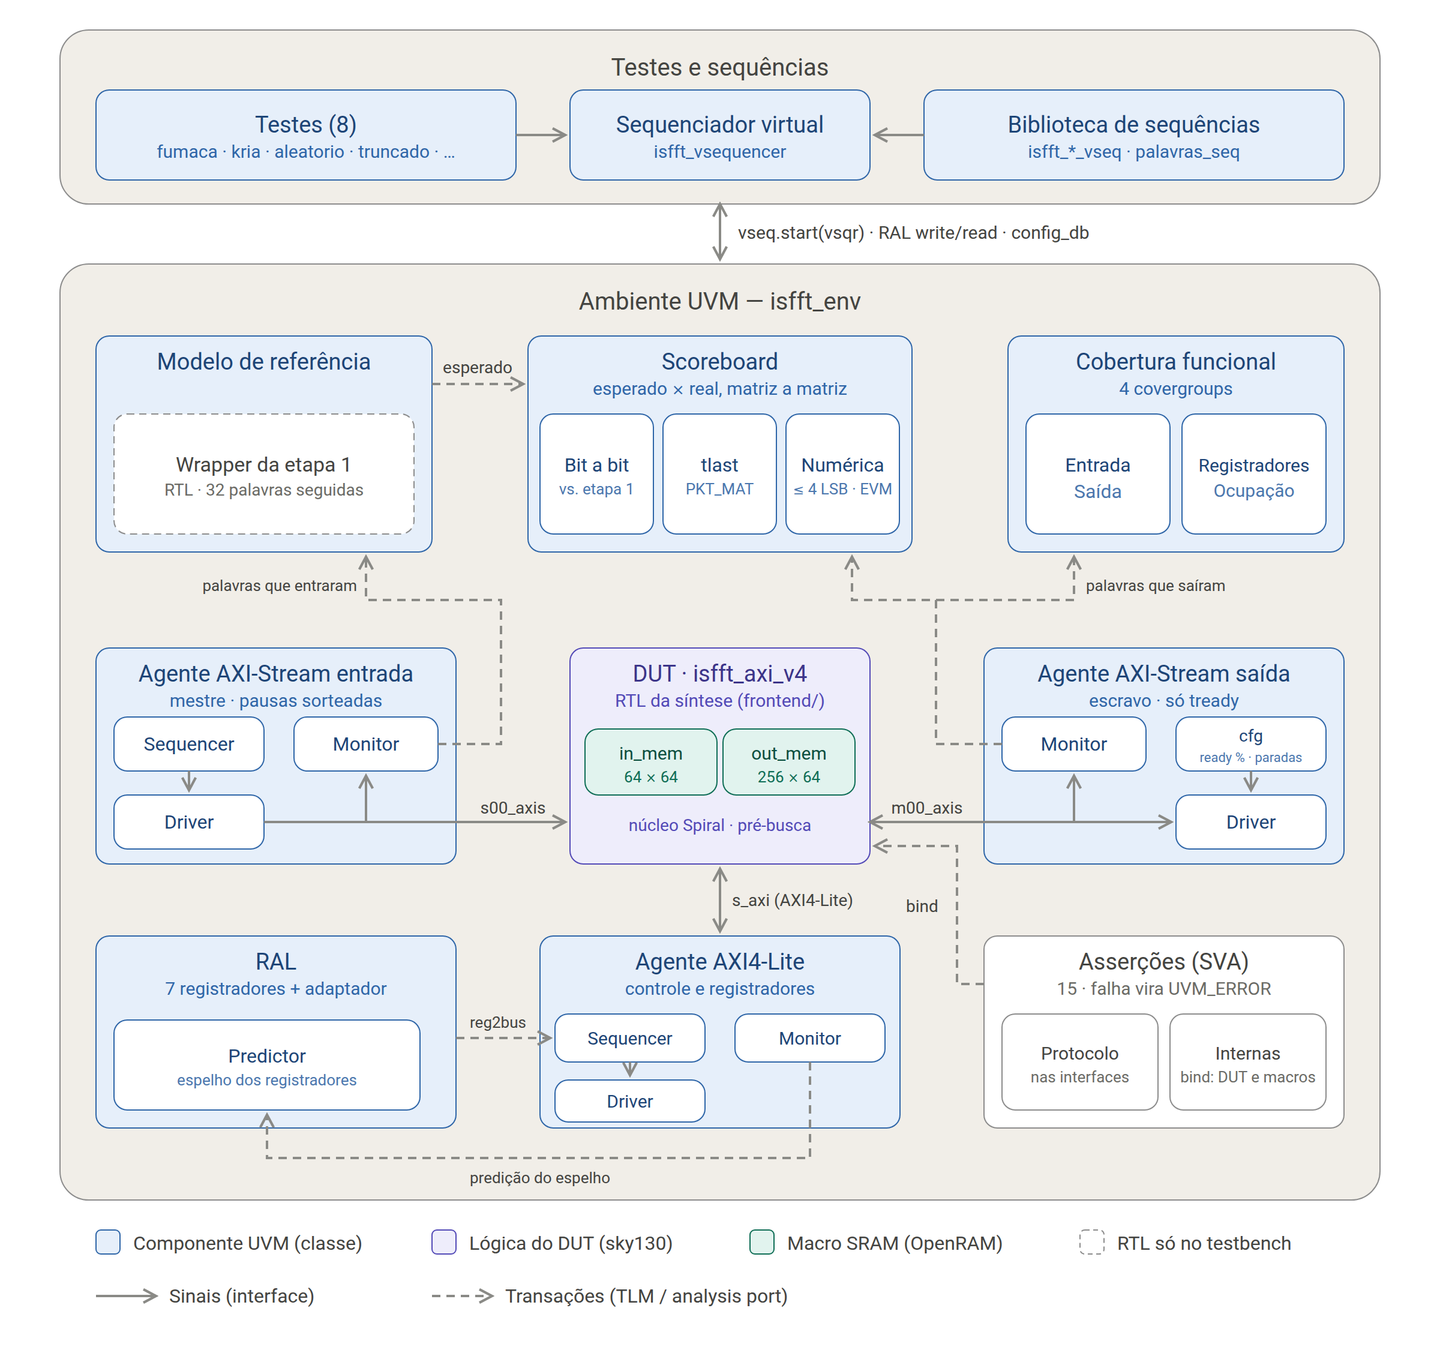
\includegraphics[width=0.46\textwidth]{Imagens/uvm_ambiente.png}}
\caption{Ambiente UVM do IP ISFFT: agentes, RAL, modelo de referência, \textit{scoreboard}, asserções e cobertura.}
\label{fig_uvm}
\end{figure}

\subsection{Resultados de Funcionalidade}
A regressão final tem 10 testes (Tabela~\ref{tab_uvm}). Todos passaram, com 0 erros de dado, 0 erros de \texttt{tlast}, 0 \texttt{UVM\_ERROR}, 0 \texttt{UVM\_WARNING} e nenhuma asserção falhando. O pior erro numérico dentro da faixa válida foi de 3,14 LSB. O teste \texttt{kria} reproduziu exatamente o EVM medido na placa.

\begin{table*}[htbp]
\caption{Regressão UVM no Xcelium 26.03 (semente 1)}
\label{tab_uvm}
\begin{center}
\begin{tabular}{|l|l|r|c|c|}
\hline
\textbf{Teste} & \textbf{Cenário} & \textbf{Palavras bit a bit} & \textbf{Pior erro numérico} & \textbf{Resultado} \\
\hline
\texttt{fumaca} & 1 matriz & 32 & 0,77 LSB & Passou \\
\texttt{registradores} & \textit{reset}, leitura/escrita, escrita em registrador RO & -- & -- & Passou \\
\texttt{kria} & 3 matrizes da placa (EVM igual ao da placa) & 96 & 1,48 LSB & Passou \\
\texttt{aleatorio} & 40 matrizes, 5 tipos $\times$ 4 amplitudes & 1.280 & 3,14 LSB & Passou \\
\texttt{truncado} & pacotes truncados, com as pontas dirigidas & 1.280 & 2,98 LSB & Passou \\
\texttt{contrapressao} & 60 matrizes, \texttt{tready} 50\% e paradas longas & 1.920 & 3,14 LSB & Passou \\
\texttt{soft\_reset} & 2 \textit{soft resets}, um com o núcleo calculando & 200 & 2,48 LSB & Passou \\
\texttt{kria\_regressao} & \textit{testbench} da Kria reescrito em UVM & 1.280 & 2,94 LSB & Passou \\
\texttt{vazao} & 80 matrizes sem pausa, \texttt{tready} 100\% & 2.560 & $\leq$ 4 LSB & Passou \\
\texttt{estouro} & 40 matrizes acima da faixa válida (só contado) & 1.280 & 40 de 40 estouram & Passou \\
\hline
\textbf{Total} & \textbf{10 testes} & \textbf{9.928} & $\leq$ \textbf{3,14 LSB} & \textbf{10/10} \\
\hline
\end{tabular}
\end{center}
\end{table*}

A verificação revelou um limite do núcleo que os testes da etapa 1 não haviam mostrado: o Spiral estoura quando $|\text{Re}|$ ou $|\text{Im}|$ da entrada passa de $32.767/\sqrt{2} \approx 23.170$, porque o estágio que multiplica pelo fator de 45° da IFFT não tem bit de guarda. A comparação bit a bit não acusa o problema, já que a referência tem o mesmo núcleo; só o modelo independente em ponto flutuante o detectou. A faixa válida da entrada foi documentada e o teste \texttt{estouro} passou a medi-la. Também se observou que o erro absoluto é de cerca de 3 LSB em qualquer amplitude, o que motivou usar um critério em LSB, e não em EVM, para sinais pequenos.

\subsection{Resultados de Cobertura}
A cobertura foi consolidada no Cadence IMC com o \textit{merge} das 10 rodadas (Fig.~\ref{fig_imc} e Tabela~\ref{tab_cov}). Os buracos encontrados na primeira medição viraram testes: uma espera curta na entrada, que só ocorre com entrada contínua e saída livre (teste \texttt{vazao}); truncamentos na primeira e na última palavra (pontas dirigidas); e um \textit{soft reset} com o núcleo em operação. A cobertura de código do \textit{wrapper} ficou em 73,5\% por dois motivos: a métrica passou a contar expressões (\texttt{\&}, \texttt{|}, \texttt{assign}), acrescentando 126 itens, e um bloco da FSM de escrita é inalcançável, pois o liberador gasta 33 ciclos por matriz e nunca emenda duas matrizes. Os modelos das macros e as asserções foram excluídos da cobertura de código, por não serem RTL do chip.

\begin{figure}[htbp]
\centerline{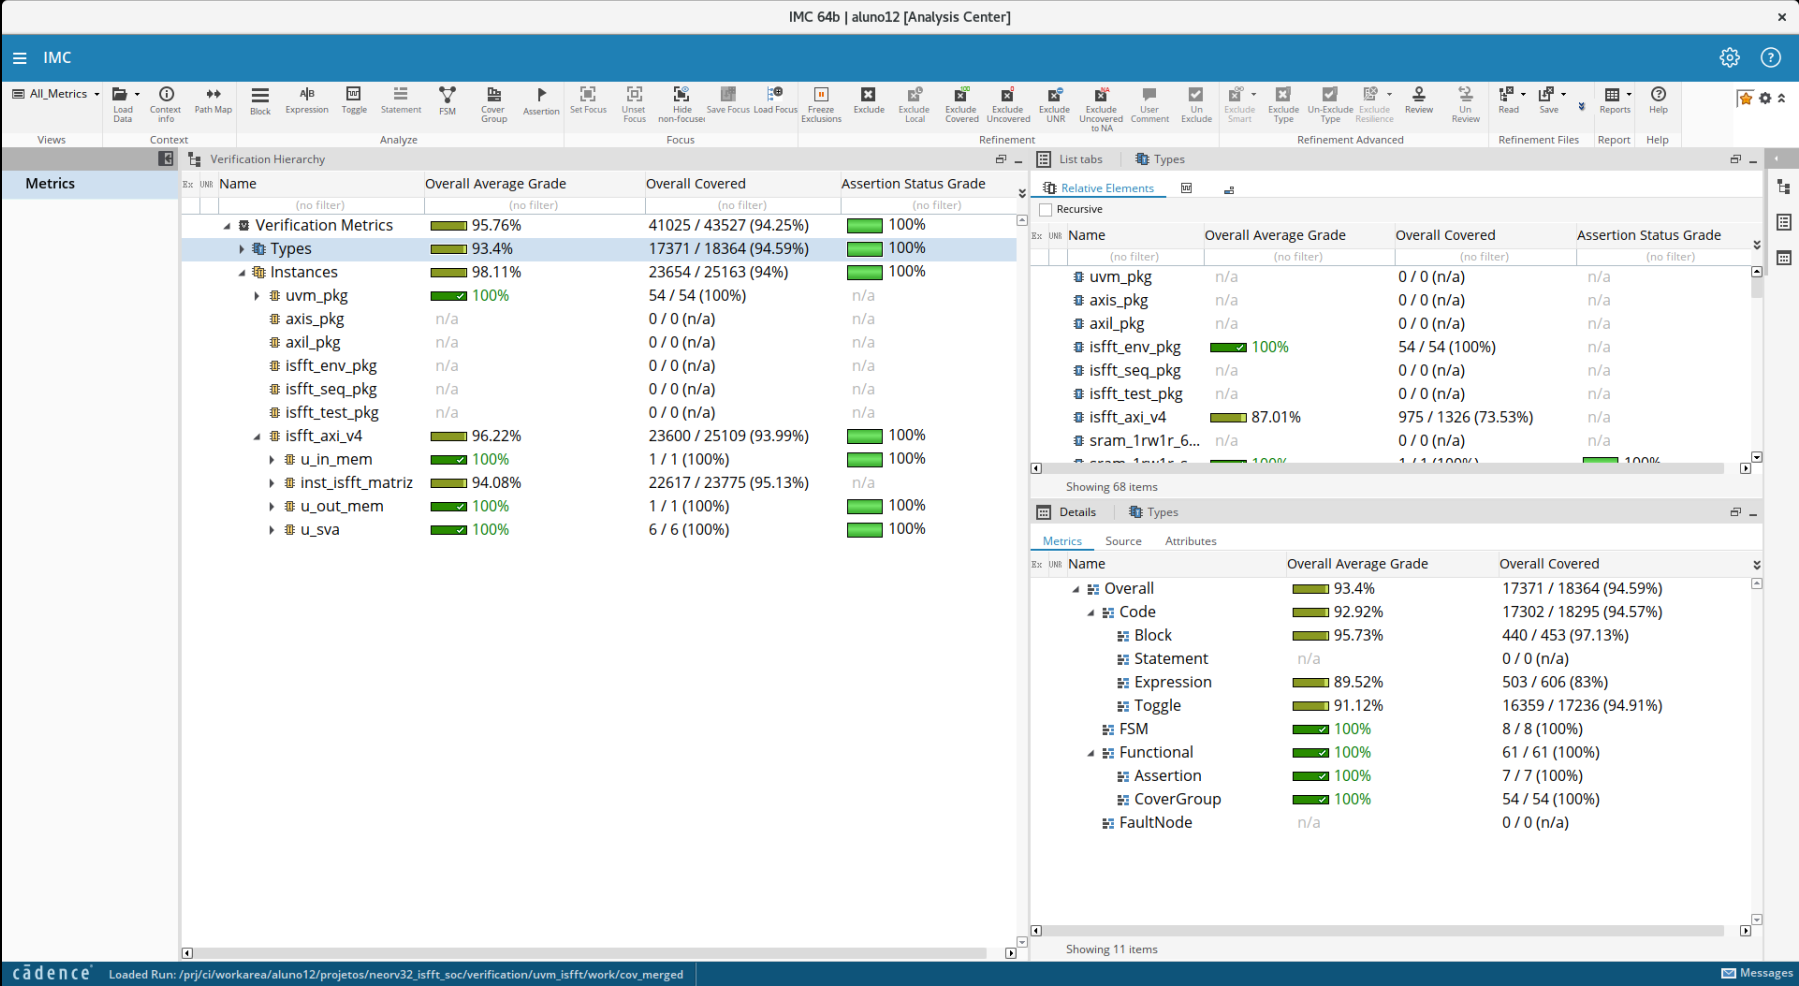
\includegraphics[width=0.48\textwidth]{Imagens/imc_cobertura.png}}
\caption{Relatório de cobertura no Cadence IMC (\textit{merge} das 10 rodadas).}
\label{fig_imc}
\end{figure}

\begin{table}[htbp]
\caption{Cobertura do IP no IMC}
\label{tab_cov}
\begin{center}
\resizebox{\columnwidth}{!}{%
\begin{tabular}{|l|c|c|}
\hline
\textbf{Métrica} & \textbf{1ª rodada (8 testes)} & \textbf{Final (10 testes)} \\
\hline
Funcional (54 \textit{bins}) & 94,4\% & \textbf{100\%} \\
Asserções & 8/8 & \textbf{8/8} \\
Código do núcleo ISFFT & 99,6\% & \textbf{100\%} (280/280) \\
Código do \textit{wrapper} & 70,7\% & \textbf{73,5\%} (975/1.326) \\
\hline
\end{tabular}%
}
\end{center}
\end{table}

% =====================================================================
\section{Fluxo DFT no IP ISFFT}

\subsection{Metodologia}
O teste de fabricação foi aplicado apenas ao IP. Na técnica de \textit{scan}, cada \textit{flip-flop} recebe um multiplexador e passa a ser um elo de uma cadeia de deslocamento: o padrão é carregado pela cadeia (\texttt{scan\_en} = 1), o circuito funciona por um ciclo (\texttt{scan\_en} = 0) e a resposta é descarregada e comparada. Com todos os \textit{flip-flops} acessíveis, a geração automática de padrões (ATPG) resolve um problema combinacional: para cada falha \textit{stuck-at}, um pino preso em 0 ou em 1, encontra valores que a ativem e propaguem até um ponto observável.

O fluxo teve cinco passos:
\begin{enumerate}
    \item Síntese com \textit{scan} completo (\textit{muxed scan}) no Genus, com 16 cadeias.
    \item Equivalência entre o RTL e o netlist com \textit{scan} no Conformal.
    \item Simulação das três matrizes no netlist com \texttt{scan\_en} = 0, para garantir que a inserção não alterou a função.
    \item ATPG \textit{stuck-at} no Modus \cite{b12}.
    \item Simulação no Xcelium dos padrões gerados aplicados ao netlist.
\end{enumerate}
Não foi necessário um sinal de modo de teste, pois o IP não tem \textit{reset} assíncrono, \textit{clock gating} nem \textit{latches}. As macros SRAM foram tratadas como caixa-preta, sem lógica de contorno.

\subsection{Resultados}
Os cinco passos foram aprovados (Tabela~\ref{tab_dft}). Os 170 padrões atingiram 99,65\% de cobertura \textit{stuck-at} no modo FULLSCAN (Tabela~\ref{tab_atpg}). As falhas restantes concentram-se em torno das macros: as 214 classificadas como possíveis ocorrem porque o padrão gera X na saída da caixa-preta, e as 151 redundantes estão em lógica sem efeito observável.

\begin{table}[htbp]
\caption{Resultados de cada passo do fluxo DFT}
\label{tab_dft}
\begin{center}
\resizebox{\columnwidth}{!}{%
\begin{tabular}{|l|l|}
\hline
\textbf{Passo} & \textbf{Resultado} \\
\hline
Síntese com \textit{scan} (Genus) & 12.552 FF, 100\% com \textit{scan}, 16 cadeias de $\sim$785 \\
LEC RTL $\times$ netlist (Conformal) & Aprovado, 0 não-equivalentes \\
Três matrizes com \texttt{scan\_en}=0 (Xcelium) & Aprovado \\
ATPG \textit{stuck-at} (Modus) & 170 padrões, 99,65\% \\
Padrões no netlist (Xcelium) & 170/170, 0 divergências em 2.156.112 comparações \\
\hline
\end{tabular}%
}
\end{center}
\end{table}

\begin{table}[htbp]
\caption{Cobertura de falhas \textit{stuck-at} no Modus}
\label{tab_atpg}
\begin{center}
\resizebox{\columnwidth}{!}{%
\begin{tabular}{|l|r|r|r|r|r|r|}
\hline
\textbf{Modo} & \textbf{Falhas} & \textbf{Testadas} & \textbf{Possíveis} & \textbf{Redund.} & \textbf{Não test.} & \textbf{Cobertura} \\
\hline
FULLSCAN & 341.871 & 340.510 & 214 & 151 & 996 & 99,65\% \\
Global & 343.063 & 340.510 & 214 & 151 & 2.188 & 99,30\% \\
\hline
\end{tabular}%
}
\end{center}
\end{table}

O custo da testabilidade está na Tabela~\ref{tab_dft_area}. A área de lógica cresce 17,2\%, porque cada \textit{flip-flop} é substituído por uma célula com o multiplexador de \textit{scan} embutido; com as duas macros, o aumento total é de 8,6\%. O IP sem \textit{scan} usado na comparação é o da síntese do SoC, com a mesma biblioteca e o mesmo RTL. A folga de \textit{setup} não é comparável entre as duas sínteses, pois as restrições do IP isolado são outras.

\begin{table}[htbp]
\caption{Custo do \textit{scan} em área}
\label{tab_dft_area}
\begin{center}
\resizebox{\columnwidth}{!}{%
\begin{tabular}{|l|r|r|r|}
\hline
 & \textbf{Sem \textit{scan}} & \textbf{Com \textit{scan}} & \textbf{Diferença} \\
\hline
Área total com 2 macros ($\mu$m$^2$) & 897.901 & 974.849 & +8,6\% \\
Somente lógica ($\mu$m$^2$) & 448.030 & 524.977 & +17,2\% \\
Instâncias & 36.375 & 35.962 & $-$413 \\
\hline
\end{tabular}%
}
\end{center}
\end{table}

% =====================================================================
\section{Prototipagem em FPGA}

\subsection{Utilização de Recursos, Temporização e Potência}
O sistema completo foi implementado na Kria KR260 \cite{b13} (Zynq UltraScale+ \textit{xck26-sfvc784-2LV-c}) a 100 MHz (Fig.~\ref{fig_device}). Todas as restrições de temporização foram atendidas, com WNS de +3,903 ns e WHS de +0,010 ns, sem caminhos violando entre 49.570 pontos de chegada. A utilização está na Tabela~\ref{tab_util}. Em relação ao Estudo Dirigido 1, o aumento vem do NEORV32 e da BRAM de 64 kB; a ISFFT sozinha usa 9,5 BRAMs.

\begin{figure}[htbp]
\centerline{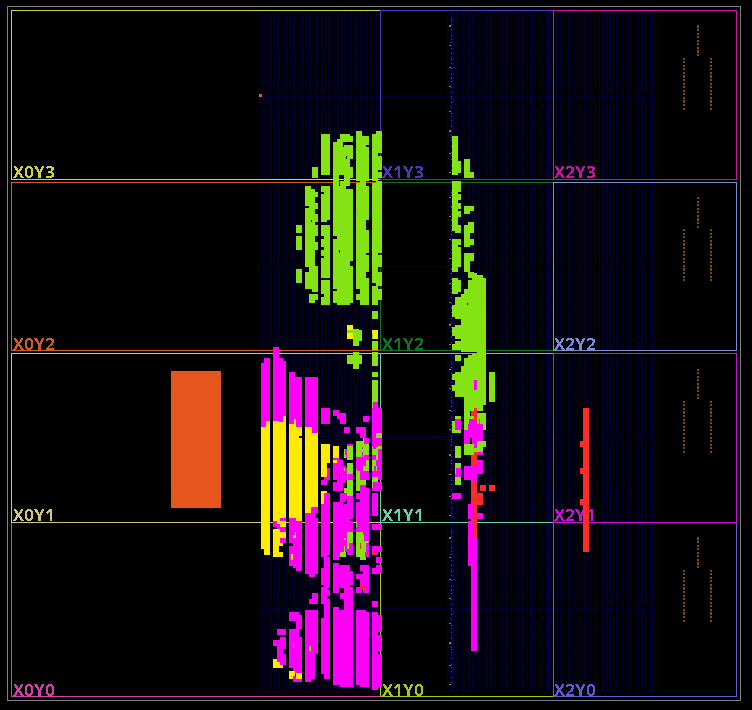
\includegraphics[width=0.36\textwidth]{Imagens/kria_dispositivo.png}}
\caption{Posicionamento do sistema NEORV32 + ISFFT no dispositivo (Vivado).}
\label{fig_device}
\end{figure}

\begin{table}[htbp]
\caption{Utilização de recursos na Kria KR260}
\label{tab_util}
\begin{center}
\begin{tabular}{|l|c|c|c|}
\hline
\textbf{Recurso} & \textbf{Utilização} & \textbf{Disponível} & \textbf{Utilização (\%)} \\
\hline
LUT & 10.376 & 117.120 & 8,86 \\
LUTRAM & 1.301 & 57.600 & 2,26 \\
FF & 15.080 & 234.240 & 6,44 \\
BRAM & 36,5 & 144 & 25,35 \\
DSP & 16 & 1.248 & 1,28 \\
\hline
\end{tabular}
\end{center}
\end{table}

A potência total estimada pelo Vivado foi de 2,846 W, dos quais 2,545 W são dinâmicos e 0,301 W estáticos. O PS consome 2,417 W (94\% da potência dinâmica), de modo que a lógica programável, incluindo o NEORV32, a ISFFT e o DMA, responde por cerca de 0,128 W de potência dinâmica.

\subsection{Validação Hardware-in-the-Loop}
O notebook Jupyter grava o firmware na BRAM, escreve na caixa de correio os endereços dos buffers e libera o NEORV32. O processador programa o DMA e a ISFFT, mede os ciclos com o contador de ciclos do RISC-V e devolve o status. A saída do hardware (Fig.~\ref{fig_output}) foi comparada com o modelo de referência (Tabela~\ref{tab_hil}): os valores de EVM são idênticos aos do Estudo Dirigido 1, agora com o RISC-V no controle. A latência do hardware foi de 506 ciclos (5,06 $\mu$s) por matriz e, incluindo a programação do DMA pelo NEORV32, de 687 ciclos (6,87 $\mu$s).

\begin{figure*}[htbp]
\centerline{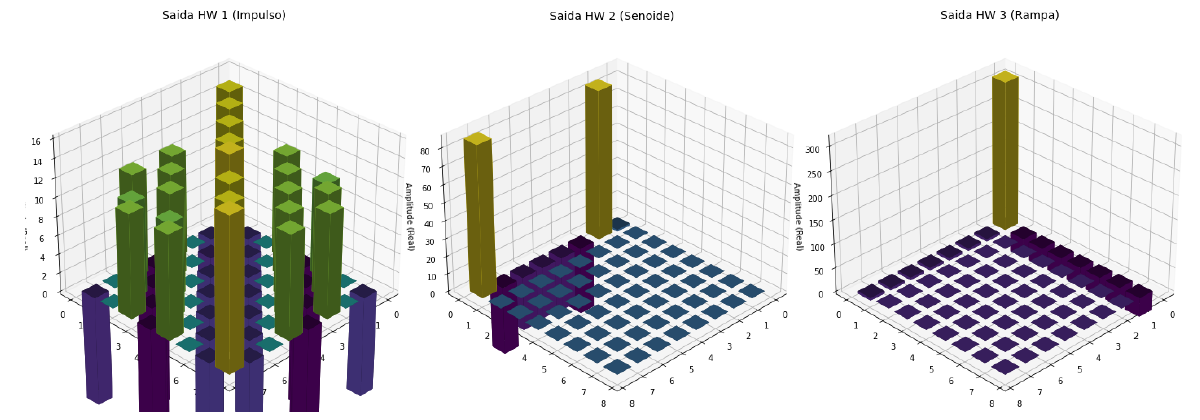
\includegraphics[width=0.85\textwidth]{Imagens/kria_saida.png}}
\caption{Saída do hardware na Kria (domínio tempo-frequência) para as três matrizes de teste, capturada pelo notebook PYNQ.}
\label{fig_output}
\end{figure*}

\begin{table}[htbp]
\caption{Resultados \textit{hardware-in-the-loop} a 100 MHz}
\label{tab_hil}
\begin{center}
\begin{tabular}{|l|c|c|c|c|}
\hline
\textbf{Matriz} & \textbf{EVM (\%)} & \textbf{MAE} & \textbf{Ciclos} & \textbf{Com DMA} \\
\hline
1 (Impulso) & 3,4122 & 0,40 & 506 & 687 \\
2 (Senoide) & 0,7822 & 0,10 & 507 & 687 \\
3 (Rampa) & 0,5965 & 0,09 & 506 & 687 \\
\hline
\end{tabular}
\end{center}
\end{table}

A latência por matriz é maior que os 320 ns do Estudo Dirigido 1 porque as métricas diferem: lá se mediu a vazão do \textit{pipeline} com várias matrizes em sequência; aqui, o tempo de ida e volta de uma matriz isolada pelo DMA, com o RISC-V programando cada transferência. Comparado ao tempo médio de 0,81 ms do modelo em Python no ARM medido no Estudo Dirigido 1 \cite{b14}, o sistema com o NEORV32 é cerca de 118 vezes mais rápido. Em energia por matriz ($E = P \times t$), a estimativa é de 0,128 W $\times$ 6,87 $\mu$s $\approx$ 0,88 $\mu$J para o caminho em hardware, contra 2,417 W $\times$ 0,81 ms $\approx$ 1,96 mJ para o ARM. Esses valores partem das estimativas de potência do Vivado, e não de medições na placa, e por isso devem ser lidos como ordem de grandeza.

% =====================================================================
\section{Fluxo ASIC no Cadence}

\subsection{Síntese Lógica}
O SoC foi sintetizado no Genus \cite{b11} com a biblioteca \texttt{sky130\_fd\_sc\_hd} no canto típico (TT, 25 °C, 1,80 V), os arquivos Liberty das quatro macros e relógio de 20 ns (50 MHz). A síntese levou cerca de 10 minutos e resultou em 1,913 mm$^2$, 60.026 instâncias (19.823 \textit{flip-flops} e 4 macros), folga de \textit{setup} de +2,41 ns e nenhuma violação de transição, capacitância ou \textit{fanout}. A distribuição de área está na Tabela~\ref{tab_area}.

\begin{table}[htbp]
\caption{Distribuição de área na síntese do SoC}
\label{tab_area}
\begin{center}
\resizebox{\columnwidth}{!}{%
\begin{tabular}{|l|r|c|}
\hline
\textbf{Bloco} & \textbf{Área ($\mu$m$^2$)} & \textbf{\% do chip} \\
\hline
Macros SRAM (4) & 1.182.838 & 61,8 \\
Lógica da ISFFT & 448.030 & 23,4 \\
\quad \textit{ping-pong} e registradores & 149.015 & 7,8 \\
\quad IFFT 1D / FFT 1D (Spiral) & 141.104 / 138.334 & 7,4 / 7,2 \\
\quad \textit{wrapper} \texttt{isfft\_axi\_v4} & 18.892 & 1,0 \\
Lógica do NEORV32 & 275.798 & 14,4 \\
\quad FIFOs do SLINK ($2 \times 64 \times 37$) & 147.333 & 7,7 \\
\quad CPU rv32imc & 97.058 & 5,1 \\
Conversores 32 $\leftrightarrow$ 64 & 6.205 & 0,3 \\
\hline
\textbf{Total} & \textbf{1.912.952} & \textbf{100} \\
\hline
\end{tabular}%
}
\end{center}
\end{table}

As memórias dominam o chip: somando as macros com as memórias que ficaram em \textit{flip-flops} (FIFOs do SLINK, \textit{ping-pong} e banco de registradores), quase 80\% da área é memória, enquanto a aritmética da FFT e da IFFT ocupa 14,6\%. Essa assinatura aparece também nas células: 89\% dos \textit{flip-flops} não têm \textit{reset} e 62\% das células combinacionais são \texttt{a22o}/\texttt{a22oi}, o multiplexador de leitura dessas memórias.

O caminho crítico está na CPU, e não na ISFFT: uma subtração de 32 bits em \textit{ripple carry} no multiplicador/divisor, com 32 somadores completos em cadeia que respondem por 12,5 ns dos 15,5 ns de atraso. Os dez piores caminhos estão todos na CPU, com cerca de 2,4 ns de folga.

\subsection{Simulação Pós-Síntese e Equivalência}
O netlist do Genus foi simulado no Xcelium com o mesmo firmware do RTL, processando as três matrizes por DMA e SLINK. Foi necessário compilar o modelo das células com as definições \texttt{FUNCTIONAL} e \texttt{UNIT\_DELAY}, porque o modelo Verilog distribuído com o PDK aberto não tem blocos \texttt{specify}; sem elas, toda a simulação ficava em X. O resultado está na Tabela~\ref{tab_post}: as três somas de verificação são iguais às do RTL (\texttt{0xeb88508e}, \texttt{0xba7fc58e} e \texttt{0xb29c0211}), com 188.195 ciclos no netlist contra 188.194 no RTL. Cada matriz leva 2.622 ciclos (52,4 $\mu$s a 50 MHz), incluindo a movimentação pelo DMA e pelo SLINK.

A equivalência formal no Conformal confirmou que o netlist implementa o mesmo circuito do RTL: 19.828 pontos equivalentes (19.823 \textit{flip-flops}, 1 saída e 4 macros), nenhum não-equivalente ou abortado, e 169 de 169 módulos aprovados.

\begin{table}[htbp]
\caption{Verificação da síntese}
\label{tab_post}
\begin{center}
\resizebox{\columnwidth}{!}{%
\begin{tabular}{|l|l|l|}
\hline
\textbf{Verificação} & \textbf{Pergunta} & \textbf{Resposta} \\
\hline
Genus & Fecha temporização? & Sim: +2,41 ns a 50 MHz \\
Conformal LEC & Netlist $\equiv$ RTL? & Sim: 169/169 módulos \\
Xcelium pós-síntese & O netlist funciona? & Sim: 3 somas = RTL \\
Simulação RTL & A matemática está certa? & Sim: EVM = placa \\
\hline
\end{tabular}%
}
\end{center}
\end{table}

\subsection{Observação sobre a Potência}
O relatório de potência do Genus não pôde ser usado. O arquivo Liberty gerado pela OpenRAM declara potência interna fora de escala, e o total estimado chega a 2.767 W. Considerando só as células padrão, a estimativa é de cerca de 50 mW, obtida sem atividade de simulação (\textit{vectorless}) e, portanto, válida apenas como ordem de grandeza. Uma estimativa confiável exige corrigir a potência das macros e usar a atividade da simulação pós-síntese.

% =====================================================================
\section{Do Netlist ao GDSII com Ferramentas Abertas (Atividade Extra)}

\subsection{Layout do Núcleo}
O netlist do Genus foi levado ao layout com o LibreLane \cite{b9}, que encadeia o OpenROAD \cite{b8} (\textit{floorplan}, rede de alimentação, posicionamento, árvore de relógio, roteamento e análise temporal), o Magic e o KLayout (GDS, DRC e comparação XOR) e o Netgen (LVS). O núcleo (\texttt{asic\_top}) tem área de $2{,}0 \times 1{,}5$ mm com as quatro macros; as etapas estão na Fig.~\ref{fig_layout}. Três problemas se destacaram:
\begin{itemize}
    \item \textbf{Congestionamento:} o excesso de demanda no roteamento global caiu de 4.682 para 0 com densidade alvo de 65\% e a DMEM movida para o canto, o que abriu o canal entre as macros.
    \item \textbf{Macros vazias no GDS:} a comparação XOR entre o Magic e o KLayout apontou 15,7 milhões de diferenças. O LEF gerado pela OpenRAM não tinha a declaração \texttt{FOREIGN}, e o KLayout gravava as macros vazias; com o LEF corrigido, as diferenças foram a zero.
    \item \textbf{Unidades do LEF:} o LEF da OpenRAM usa 2000 unidades por mícron, enquanto o OpenROAD só aceita 1000 no sky130, o que exigiu uma conversão.
\end{itemize}

\begin{figure*}[htbp]
\centerline{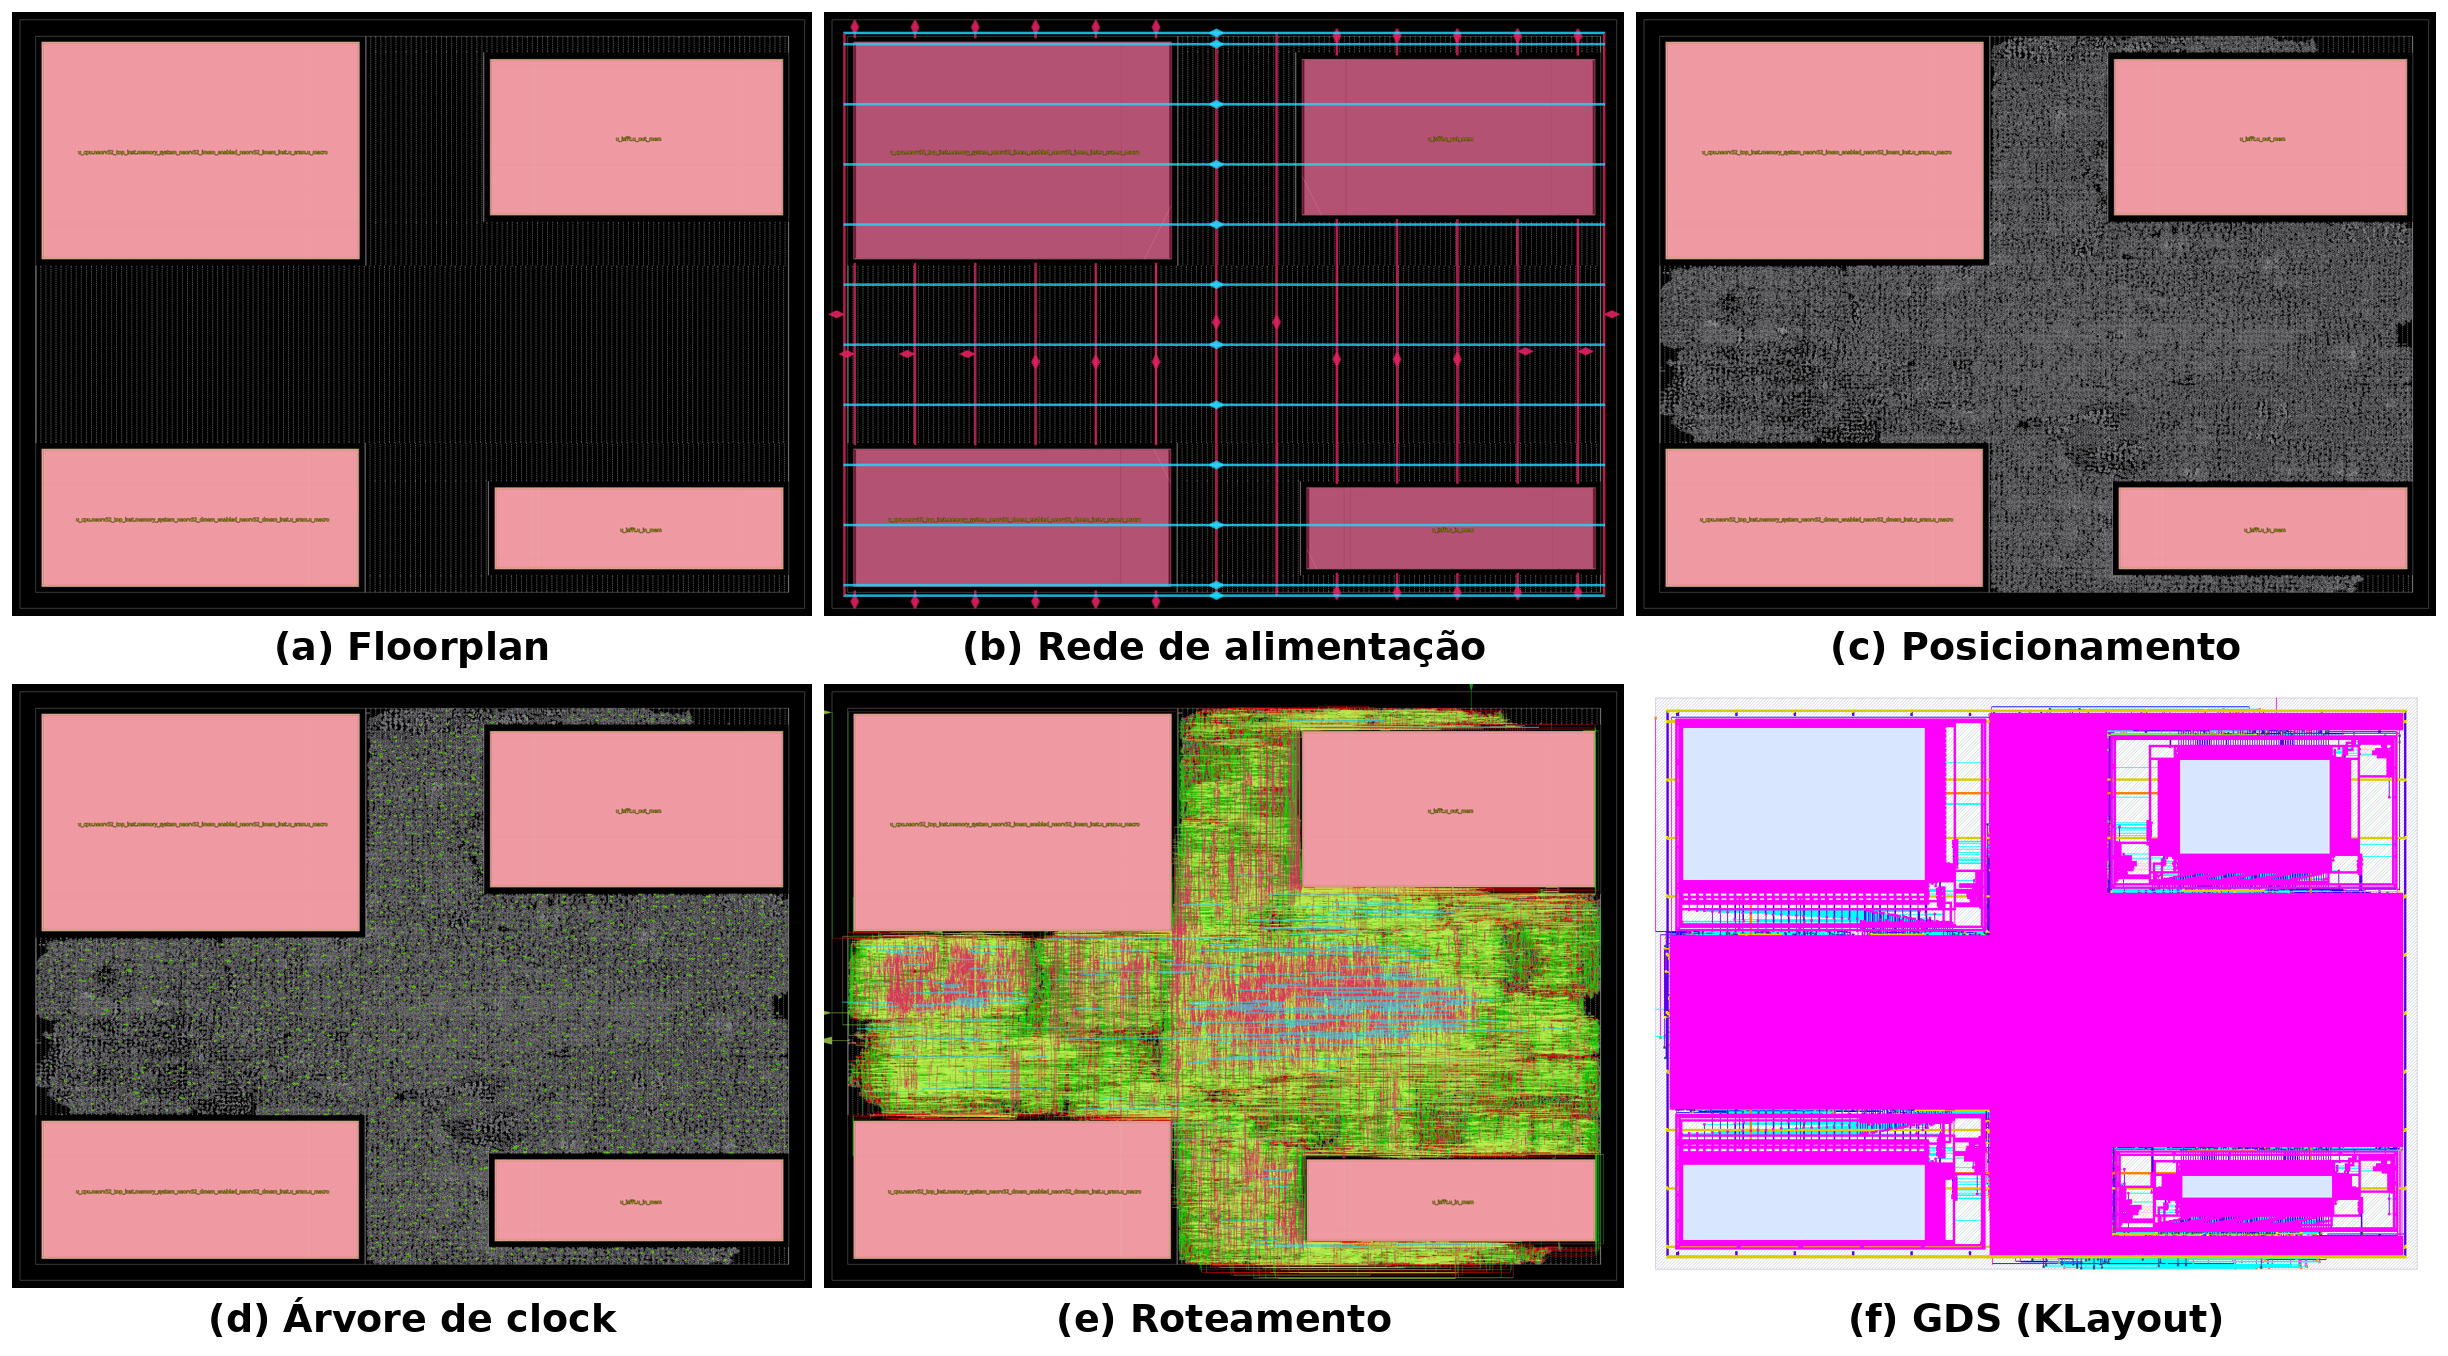
\includegraphics[width=0.92\textwidth]{Imagens/layout_nucleo_etapas.png}}
\caption{Etapas do layout do núcleo no LibreLane: (a) \textit{floorplan} com as macros, (b) rede de alimentação, (c) posicionamento, (d) árvore de relógio, (e) roteamento e (f) GDS final no KLayout.}
\label{fig_layout}
\end{figure*}

\subsection{Chip com o Anel de Pads}
No segundo nível, o núcleo entrou como macro dentro de um anel de \textit{pads} \texttt{sky130\_ef\_io}, em uma área de $2{,}70 \times 2{,}20$ mm (Fig.~\ref{fig_chip}). São 11 \textit{pads}: 4 de sinal (\texttt{clk}, \texttt{rstn}, \texttt{rx} e \texttt{tx}), 6 de alimentação e 1 fatia, além de 4 cantos. A primeira versão apresentou transição de 3,54 ns no \textit{pad} \texttt{tx}, acima do limite de 1,5 ns. Com o modelo de tempo do núcleo disponível no nível do chip, o reparo do OpenROAD inseriu um \textit{buffer} antes do \textit{pad}, e a transição caiu para 0,11 ns.

\begin{figure}[htbp]
\centerline{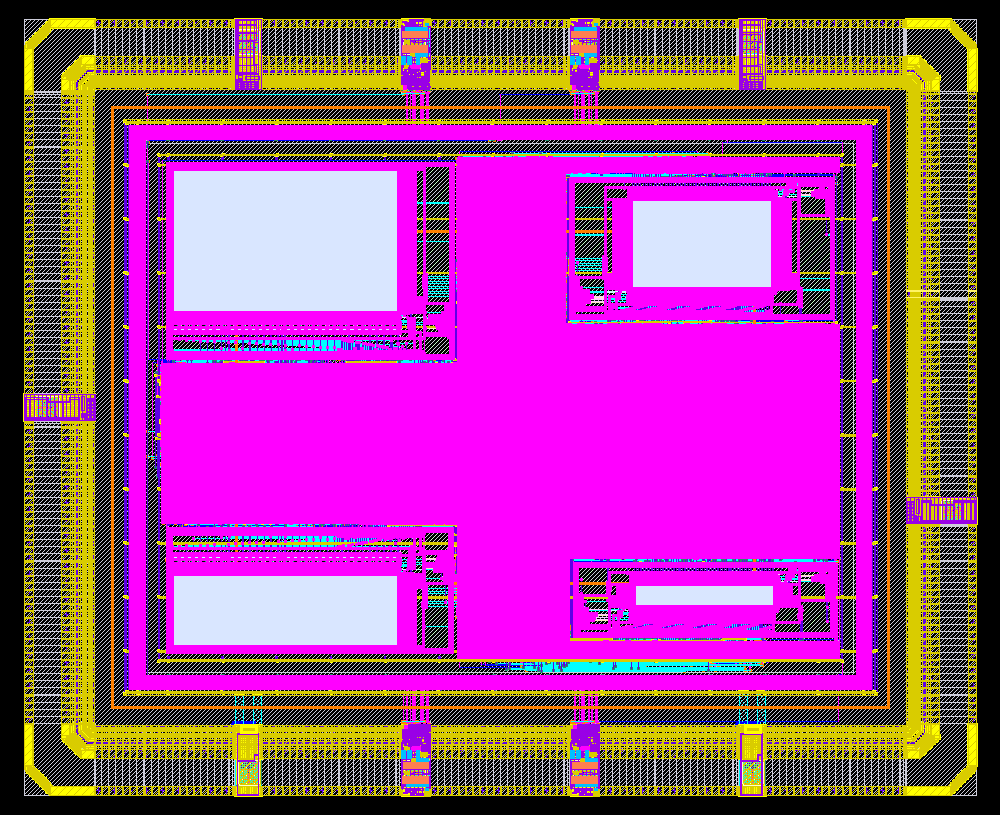
\includegraphics[width=0.46\textwidth]{Imagens/chip_final.png}}
\caption{Chip final com o anel de \textit{pads} e o preenchimento de metal.}
\label{fig_chip}
\end{figure}

\subsection{Verificação Final}
A Tabela~\ref{tab_signoff} resume a verificação nos dois níveis. No núcleo, os 130 erros de DRC restantes estão em pinos sem uso das macros, tratadas como caixa-preta. No chip, a faixa dos \textit{pads} foi isenta, porque os erros apontados estão nas próprias células de E/S da \textit{foundry}. A equivalência entre o netlist do layout e o do Genus e a simulação com o firmware fecham a cadeia: RTL $\equiv$ Genus $\equiv$ layout (LEC) $\equiv$ GDS (LVS), e o desenho executa o firmware corretamente.

\begin{table*}[htbp]
\caption{Verificação final do layout}
\label{tab_signoff}
\begin{center}
\begin{tabular}{|l|l|l|}
\hline
\textbf{Verificação} & \textbf{Núcleo (\texttt{asic\_top})} & \textbf{Chip com o anel de \textit{pads}} \\
\hline
DRC (Magic) & 0 erros reais (130 isentos: pinos sem uso das macros) & 0 no desenho (faixa dos \textit{pads} isenta) \\
LVS (Netgen) & \textit{Circuits match uniquely} & \textit{Circuits match uniquely} \\
XOR Magic $\times$ KLayout & 0 & 0 \\
Antena & 0 & 0 \\
LEC: netlist do layout $\times$ Genus & 19.828 pontos equivalentes & -- \\
Simulação com o firmware & 3 somas = RTL & 3 somas = RTL \\
STA \textit{setup} (50 MHz) & +0,32 ns (TT) & +2,95 ns (TT); +2,37 ns no pior caso (SS) \\
STA \textit{hold} & +0,13 ns (TT); 15 caminhos até $-$28 ps no canto FF (aceitos) & +3,63 ns \\
\hline
\end{tabular}
\end{center}
\end{table*}

% =====================================================================
\section{Conclusão e Próximos Passos}

Este trabalho integrou o acelerador ISFFT ao processador RISC-V NEORV32 e o validou em três níveis. No nível do \textbf{bloco}, o IP foi verificado com UVM (10 de 10 testes, 100\% de cobertura funcional, 8 de 8 asserções), e a verificação revelou e documentou um limite de estouro do núcleo que os testes anteriores não haviam mostrado. O IP também se tornou testável, com 99,65\% de cobertura \textit{stuck-at} ao custo de 17,2\% de área de lógica. No nível do \textbf{sistema}, o NEORV32 controla sozinho o DMA e a ISFFT na Kria KR260, com latência de 6,87 $\mu$s por matriz e o mesmo EVM do modelo de referência. No nível do \textbf{silício}, o SoC foi sintetizado em SkyWater 130 nm com 1,91 mm$^2$ a 50 MHz, com equivalência formal e simulação pós-síntese idêntica ao RTL, e foi levado até o GDSII com o anel de \textit{pads}, com DRC e LVS limpos.

O fio condutor do projeto foi usar sempre o mesmo estímulo: o EVM de 3,41/0,78/0,60\% se repetiu na placa, na simulação RTL do SoC e no UVM, e as mesmas três somas de verificação se repetiram do RTL ao netlist do layout. Os próximos passos, no Trabalho de Conclusão de Curso, são:
\begin{itemize}
    \item \textbf{Transceptor completo:} substituir a cadeia ISFFT + Heisenberg pela Transformada Inversa de Zak no transmissor e implementar o receptor.
    \item \textbf{Escalabilidade:} crescer a matriz rumo a $1024 \times 256$, compatível com enlaces LEO, respeitando a faixa válida de entrada identificada pelo UVM.
    \item \textbf{Protótipo real:} migrar para a ZCU102 com o AD-FMCOMMS3 (AD9361) e realizar transmissão \textit{over-the-air} entre duas placas.
\end{itemize}

\begin{thebibliography}{00}
\bibitem{b1} R. Hadani et al., ``Orthogonal Time Frequency Space Modulation,'' in IEEE WCNC, 2017.
\bibitem{b2} MathWorks, ``OTFS Modulation,'' Documentation. [Online]. Disponível: \url{https://www.mathworks.com/help/comm/ug/otfs-modulation.html}.
\bibitem{b3} E. Viterbo, ``OTFS Modulation,'' Monash University, 2019. [Online]. Disponível: \url{https://users.monash.edu/~gfarr/research/slides/Viterbo_Nov_2019___OTFS_modulation.pdf}.
\bibitem{b4} Spiral, ``DFT Hardware Generator,'' [Online]. Disponível: \url{https://www.spiral.net/hardware/dftgen.html}.
\bibitem{b5} S. Nolting, ``The NEORV32 RISC-V Processor,'' [Online]. Disponível: \url{https://github.com/stnolting/neorv32}.
\bibitem{b6} Google e SkyWater Technology, ``SkyWater SKY130 Open Source PDK,'' [Online]. Disponível: \url{https://github.com/google/skywater-pdk}.
\bibitem{b7} M. R. Guthaus et al., ``OpenRAM: An Open-Source Memory Compiler,'' in IEEE/ACM ICCAD, 2016.
\bibitem{b8} T. Ajayi et al., ``Toward an Open-Source Digital Flow: First Learnings from the OpenROAD Project,'' in ACM/IEEE DAC, 2019.
\bibitem{b9} LibreLane, ``LibreLane: ASIC implementation flow,'' [Online]. Disponível: \url{https://github.com/librelane/librelane}.
\bibitem{b10} Accellera Systems Initiative, ``Universal Verification Methodology (UVM) 1.1d Class Reference,'' 2013.
\bibitem{b11} Cadence Design Systems, ``Genus Synthesis Solution User Guide.''
\bibitem{b12} Cadence Design Systems, ``Modus DFT Software Solution User Guide.''
\bibitem{b13} AMD, ``Kria KR260 Robotics Starter Kit,'' [Online]. Disponível: \url{https://www.amd.com/en/products/system-on-modules/kria/k26/kr260-robotics-starter-kit.html}.
\bibitem{b14} L. A. da Silva, ``Projeto e implementação de um módulo ISFFT para modulação OTFS em fluxos de FPGA e ASIC,'' relatório do Estudo Dirigido 1, Programa CI Digital, 2026.
\end{thebibliography}

\end{document}
